\documentclass[9pt, conference]{IEEEtran}
\IEEEoverridecommandlockouts

\usepackage{amsmath,amsfonts,graphicx}
\usepackage{amssymb,textcomp,mathtools}
\usepackage{bm,upgreek,algorithm,hyperref}
\usepackage{multirow,booktabs,hhline,array}
\usepackage{cite,url,makecell,setspace}
\usepackage{xcolor}
\pdfoutput=1

\def\thline{\noalign{\hrule height 1.0pt}}
\def\tthline{\noalign{\hrule height 1.4pt}}
\DeclareMathOperator*{\argmin}{argmin}
\DeclareMathOperator*{\argmax}{argmax}

\renewcommand{\vec}[1]{\bm{\mathrm{#1}}}
\def\x{{\mathbf x}}
\def\L{{\cal L}}

\title{Apollo: Band-sequence Modeling for High-Quality Audio Restoration}

\author{\IEEEauthorblockN{Kai~Li$^{\spadesuit,\clubsuit,*}$, Yi Luo$^{\clubsuit,*}$\\}
\IEEEauthorblockA{$^\spadesuit$Department of Computer Science and Technology, Tsinghua University, Beijing, China \\
$^\clubsuit$Tencent AI Lab, Shenzhen, China \\
tsinghua.kaili@gmail.com, oulyluo@tencent.com}
\thanks{$*$ The work was done while Yi Luo was at Tencent AI Lab and Kai Li was an intern there.}
}

\begin{document}
\maketitle

\begin{abstract}
\begin{abstract}
There is a widely-spread claim that GANs are difficult to train, and GAN architectures in the literature are littered with empirical tricks. We provide evidence against this claim and build a modern GAN baseline in a more principled manner. First, we derive a well-behaved regularized relativistic GAN loss that addresses issues of mode dropping and non-convergence that were previously tackled via a bag of ad-hoc tricks. We analyze our loss mathematically and prove that it admits local convergence guarantees, unlike most existing relativistic losses. Second, this loss allows us to discard all ad-hoc tricks and replace outdated backbones used in common GANs with modern architectures. Using StyleGAN2 as an example, we present a roadmap of simplification and modernization that results in a new minimalist baseline---\modelName (``Re-GAN''). Despite being simple, our approach surpasses StyleGAN2 on FFHQ, ImageNet, CIFAR, and Stacked MNIST datasets, and compares favorably against state-of-the-art GANs and diffusion models.\\
Code: \href{https://www.github.com/brownvc/R3GAN}{https://www.github.com/brownvc/R3GAN}
\end{abstract}
\end{abstract}
\begin{IEEEkeywords}
Audio restoration, audio superresolution, bandwidth extension, generative adversarial network 
\end{IEEEkeywords}
\section{Introduction}
\label{sec:introduction}
%
\section{Introduction}
%
% Problem
Time series modeling is a well-established problem, with tasks such as forecasting and classification motivated by many domains such as healthcare, finance, and engineering~\citep{shumway2000time}. 
% Furthermore, time series data is diverse and readily available, presenting an exciting modality to learn from.
% Why interesting, important, and hard
However, effective time series modeling presents several challenges: 
% Methods often must be expressive, able to forecast arbitrary horizons, and efficient.
% itemsep=0.1pt,
\begin{itemize}[leftmargin=*]
% \begin{itemize}[itemsep=0.1pt, topsep=0pt,leftmargin=*]
\item First, 
% to effectively model time series data, 
methods should \textbf{expressively} capture complex, long-range, and \emph{autoregressive} dependencies. 
Time series data often reflects higher order dependencies, seasonality, and trends, governing how past samples determine future terms~\citep{chatfield2000time}. 
This motivates many classical approaches 
% and deep learning methods~\citep{zhou2022film, zhou2022fedformer, woo2022etsformer} 
that model these properties~\citep{box1970time, winters1960forecasting}, alongside expressive deep learning mechanisms such as attention~\citep{vaswani2017attention} and fully connected layers that model interactions between \emph{every} sample in an input sequence~\citep{zeng2022transformers}.
%
\item Second, 
% for forecasting, 
methods
% to tackle a wide range of time series data domains and tasks, 
% methods
should be able to forecast a wide range of \textbf{long horizons} over various data domains. 
% \eg{} to handle various forecasting horizons,
% and data domains,  
% methods should be (ii) \emph{broadly and easily applicable}, 
% without costly manual oversight or overly-specialized architectural changes. 
% without costly or overspecialized architectural changes. 
Reflecting real world demands, popular forecasting benchmarks evaluate methods on
% across 58 datasets with individual target horizons~\citep{godahewa2021monash} or 
\numberMonashTasks{} different tasks~\citep{godahewa2021monash} and 24$-$960 time-step horizons~\cite{zhou2021informer}. 
Furthermore, as testament to accurately learning time series processes, 
% as a test for learning time series,
forecasting methods should ideally
% should thus handle long horizons, and ideally 
% continuously 
also be able to predict future time-steps on horizons they were not explicitly trained on.
% ideally without the need for additional retraining and architectural adaptation. 
% with fixed input sequences. 
% Classification and forecasting methods should generalize to various datasets.
%
\item Finally, methods should be \textbf{efficient} with training and inference. Many time series applications require processing very long sequences, \eg{} classifying audio data with sampling rates up to $16{,}000$ Hz \citep{warden2018speech}. 
To handle such settings---where we still need large enough models that can expressively model this data---training and inference should ideally scale \emph{subquadratically} with sequence length and model size in time and space complexity.
% Efficient training over long sequences is a fundamental challenge for deep learning, where popular Transformers 
%To thus effectively learn from such time series on modern hardware, we require fast inference that fits memory constraints.
\end{itemize}

% Why prior stuff isn't sufficient
Unfortunately, existing time series methods struggle to achieve all three criteria.  
%
Classical methods (\cf{} ARIMA~\citep{box1970time}, exponential smoothing (ETS)~\citep{winters1960forecasting}) often require manual data preprocessing and model selection to identify expressive-enough models. 
%To effectively scale across all such evaluations, we ideally can avoid added complexities with a single simple architecture.
%
Deep learning methods commonly train to predict specific horizon lengths, \ie{} as \emph{direct multi-step forecasting}~\citep{https://doi.org/10.1111/j.1467-6419.2007.00518.x}, and we find this hurts their ability to forecast longer horizons (Sec. \ref{sec:empirical_horizons}).  
% On applicability, 
% state-of-the-art neural nets often introduce specialized architectures to handle specific data properties~\citep{liu2022pyraformer,zhou2022film}. 
%
They also face limitations achieving high expressivity \emph{and} efficiency. Fully connected networks (FCNs) such as NLinear \cite{zeng2022transformers} scale quadratically in $\mathcal{O}(\ell h)$ space complexity (with input length $\ell$ and forecast length $h$). 
%
Recent Transformer-based models reduce this complexity to $\mathcal{O}(\ell + h)$, but do not always outperform the aforementioned fully connected networks on forecasting benchmarks~\citep{liu2022pyraformer, zhou2021informer}. 
%

% , despite introducing various specific architectures to improve expressiveness or efficiency~\citep{ zhou2022film, zhou2022fedformer, woo2022etsformer}.
% However, they rarely obtain higher MSE over FCNs on benchmarks, and introduce various specific architectures and processing steps.


% Deep learning methods may be highly expressive but are either non-generic by adding specialized architectures to deal with different data properties (\eg{} trends, seasonality) and tasks (\eg{} classification, forecasting, forecasting with different horizons) or are not efficient at processing long sequences. For example, fully-connected networks in \cite{zeng2022transformers} are highly expressive and achieve state-of-the-art results on many forecasting benchmarks; however, their time and space complexity scales quadratically in input sequence length and forecast horizon length. Transformer variations bring down this complexity to near linear in compute and memory~\citep{liu2022pyraformer, zhou2021informer}; however, they rarely obtain higher MSE over FCNs on benchmarks, and introduce various specific architectures and processing steps~\citep{zhou2022film, zhou2022fedformer, woo2022etsformer}.

\begin{figure}[!t]
  \centering
%   \includegraphics[width=1\textwidth]{_ICLR2023_paper/figures/figure_pull_2layer_v1.2.pdf}
  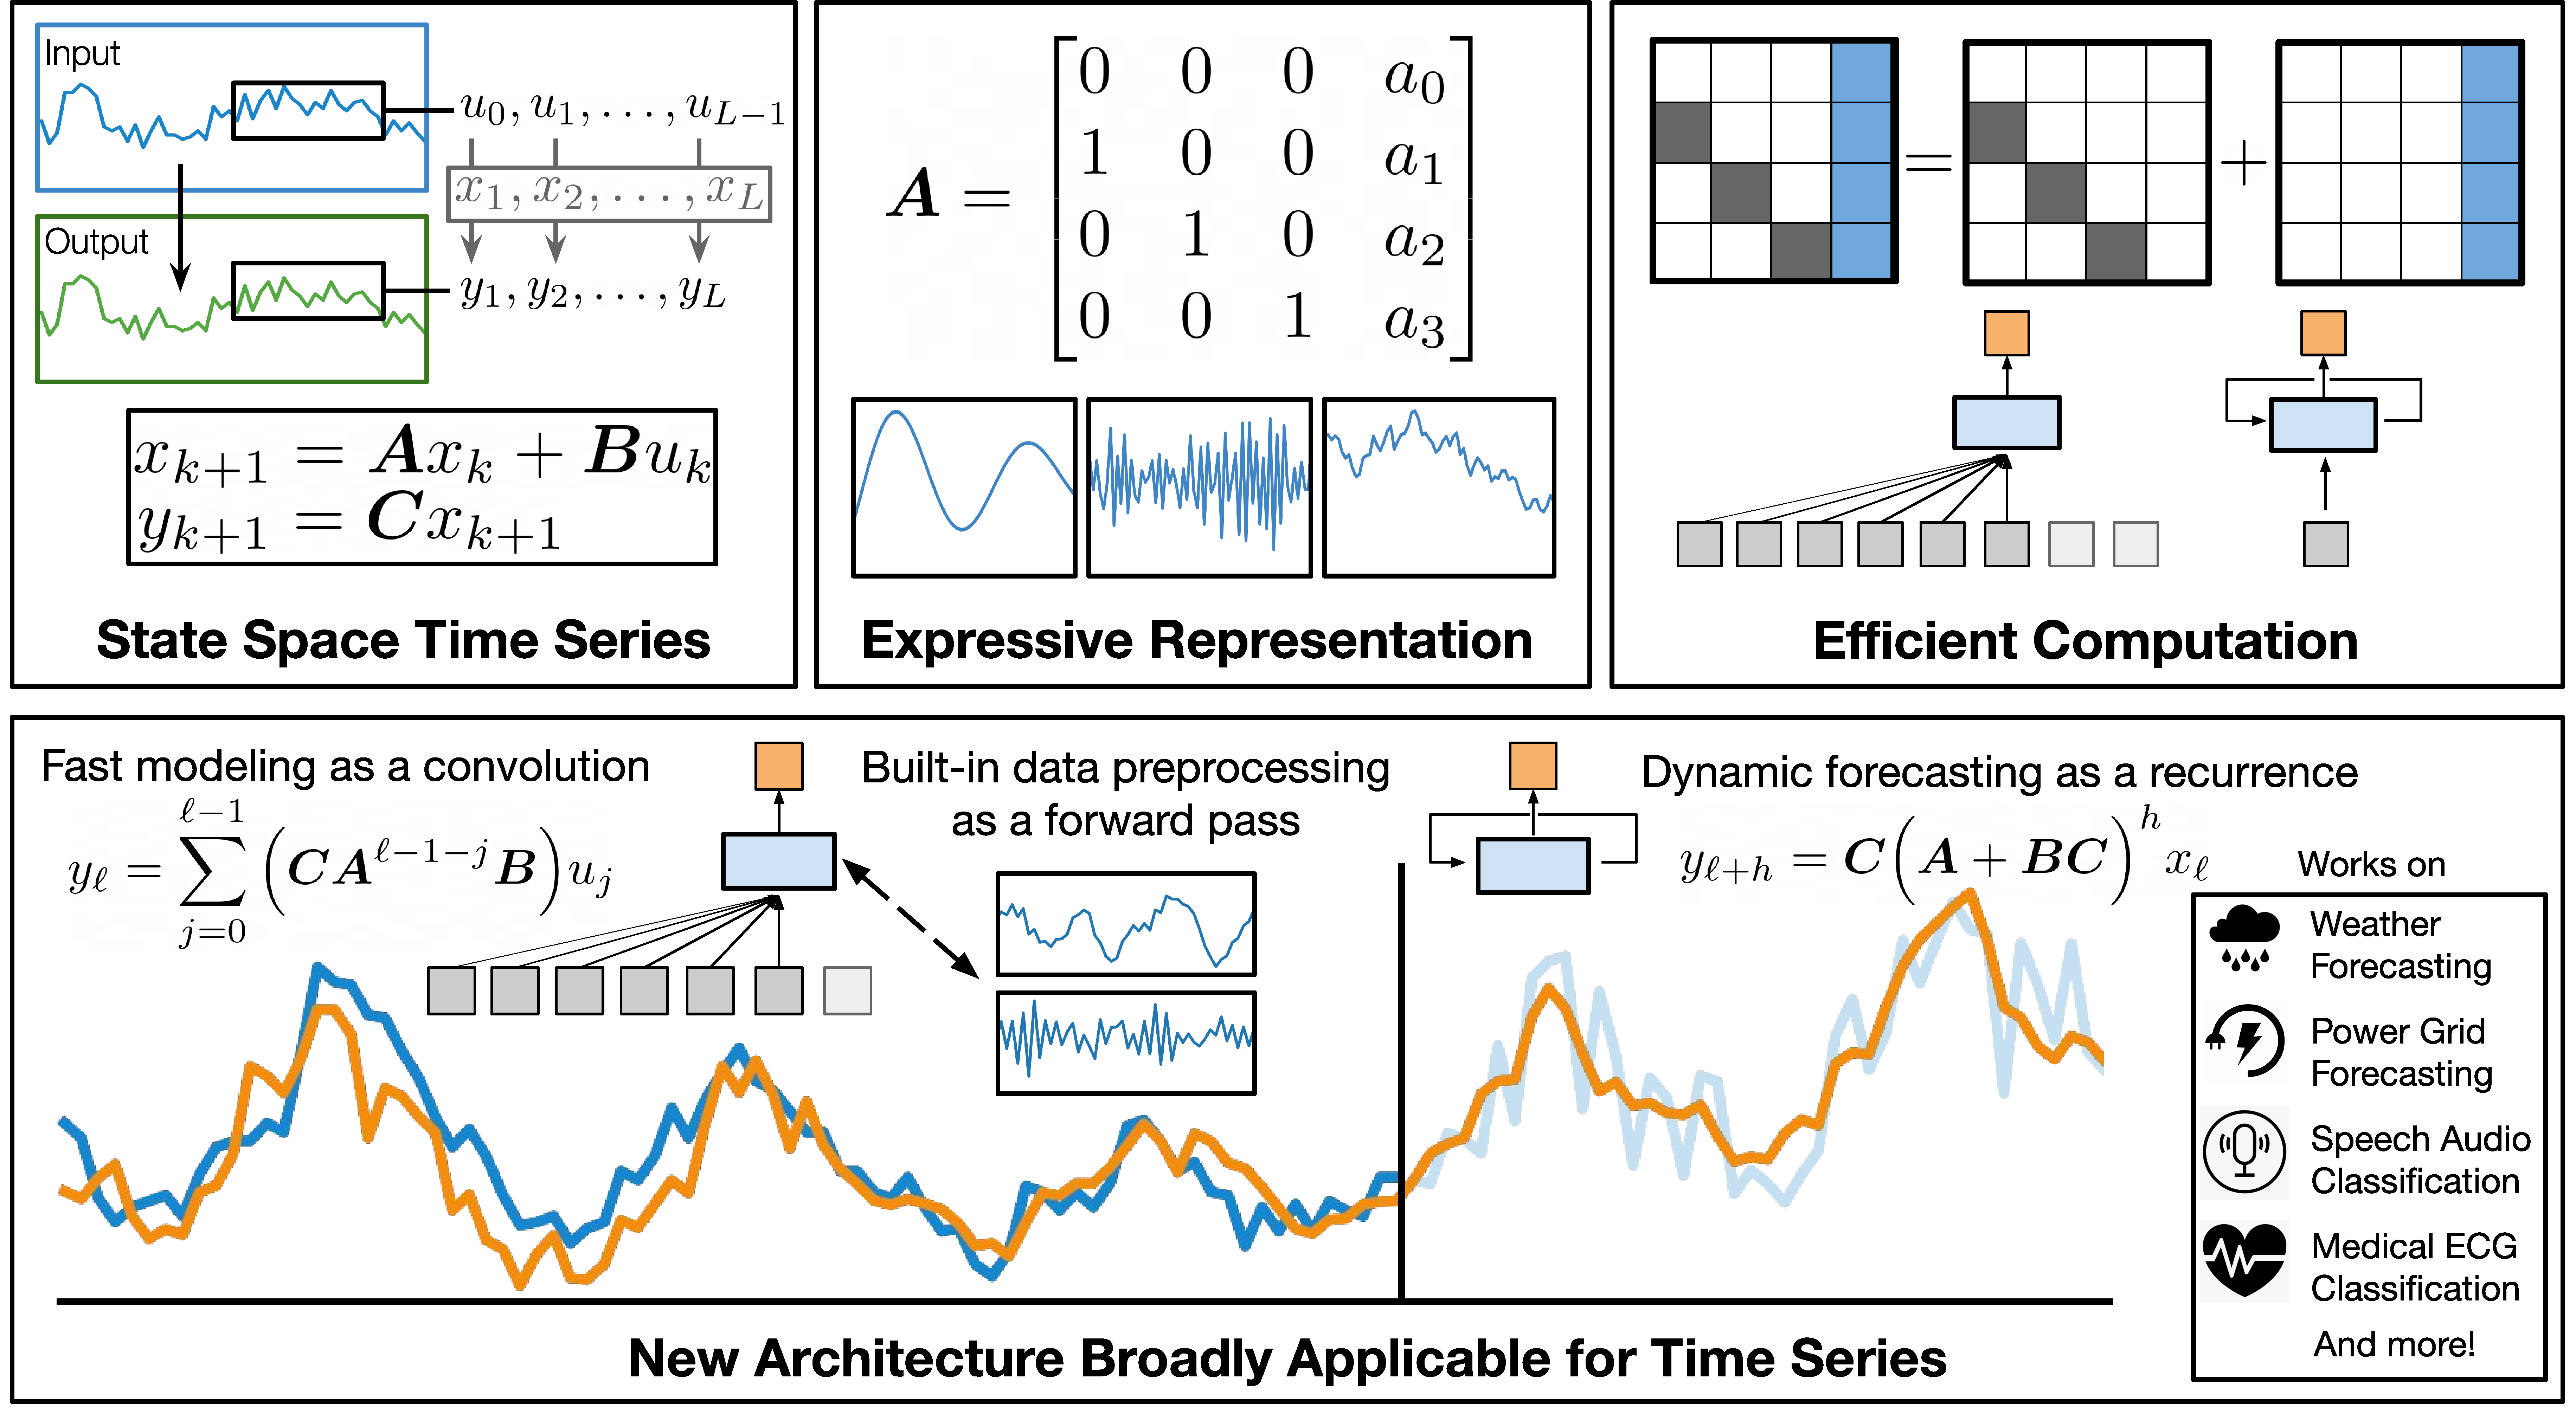
\includegraphics[width=1\textwidth]{_ICLR2023_paper/figures/time_series_ssm_use_this_2_levels_refactor1.pdf}
 \caption{We learn time series processes as state-space models (SSMs) (\textbf{top left}). We represent SSMs with the \textit{companion matrix}, which is a highly expressive representation for discrete time series  (\textbf{top middle}), and compute such SSMs efficiently as convolutions or recurrences via a shift + low-rank decomposition (\textbf{top right}). We use these SSMs to build \ourmethod{}, a new time series architecture broadly effective across tasks and domains (\textbf{bottom}).}
  \label{fig:overvew_fig1}
\end{figure}

% Our Method
%
% We thus propose \textbf{\ourmethod{}}, a new deep learning time series architecture. 
%
% Towards more effective time series modeling, 



We thus propose \textbf{\textsc{SpaceTime}}, a deep state-\textbf{space} architecture for effective \textbf{time} series modeling. 
% For more accurate forecasting and classification, 
To achieve this,
we focus on improving each criteria via three core contributions:

% \begin{enumerate}[itemsep=0.1pt,topsep=0pt,leftmargin=*]
\begin{enumerate}[topsep=0pt,leftmargin=*]
    \item For expressivity, our key idea and building block is a linear layer that models time series processes as \emph{state-space models} (SSMs) via the \emph{companion matrix} (Fig.~\ref{fig:overvew_fig1}). 
    We start with SSMs due to their connections to both classical time series analysis~\citep{kalman1960new, hamilton1994state} and recent deep learning advances~\citep{gu2021efficiently}. Classically, many time series models such as ARIMA and exponential smoothing (ETS) can be expressed as SSMs~\citep{box1970time, winters1960forecasting}. 
    Meanwhile, recent state-of-the-art deep sequence models~\citep{gu2021efficiently} have used SSMs to outperform Transformers and LSTMs on challenging long-range benchmarks~\citep{tay2020long}.
    % Meanwhile, recent SSM-based deep learning models~\citep{gu2021efficiently} have achieved state-of-the-art sequence modeling on challenging long-range benchmarks~\citep{tay2020long}. 
    Their primary innovations show how to formulate SSMs as neural network parameters that are practical to train. However, we find limitations with these deep SSMs for time series data. While we build on their advances, we prove that these prior SSM representations~\citep{ gu2021combining, gu2021efficiently, gupta2022diagonal}
    % cite these later: rangapuram2018, salinas2020deepar, lin2021ssdnet,
    cannot capture autoregressive processes fundamental for time series. We thus specifically propose the companion matrix representation for its expressive and memory-efficient properties. 
    We prove that the companion matrix SSM recovers fundamental autoregressive (AR) and smoothing processes modeled in classical techniques such as ARIMA and ETS, while only requiring $\mathcal{O}(d)$ memory to represent an $\mathcal{O}(d^2)$ matrix. 
    Thus, \ourmethod{} inherits the benefits of prior SSM-based sequence models, while introducing improved expressivity that 
    recovers fundamental time series processes
    % apture multiple AR processes and data preprocessing techniques 
    simply through its layer weights. 
    
    \item 
    % For forecasting over long horizons, we introduce a new ``closed-loop'' view of SSMs. Previous architectures apply the SSM in an ``open-loop'' fashion \citep{gu2021efficiently}, where the output is driven by the input sequence. 
    % However, to continuously forecast to long horizons, we require that the SSM has the ability to continue forecasting the signal in the absence of an input at those time steps. 
    % Inspired by classical closed-loop control~\citep{doyle2013feedback,aastrom2021feedback}, we propose a new variant of SSMs that explicitly models the next time-step input, which enables a multi-layer \ourmethod{} network to recurrently output long horizons.
    For forecasting long horizons, we introduce a new ``closed-loop'' view of SSMs. Prior deep SSM architectures either apply the SSM as an ``open-loop'' \citep{gu2021efficiently}, where fixed-length inputs necessarily generate same-length outputs, or use closed-loop autoregression where final layer outputs are fed through the \emph{entire} network as next-time-step inputs~\citep{goel2022s}. 
    We describe issues with both approaches in Sec.~\ref{sec:forecasting_ssm}, and instead achieve autogressive forecasting in a deep network with only a single SSM layer. We do so by explicitly training the SSM layer to predict its next time-step \emph{inputs}, alongside its usual outputs. This allows the SSM to recurrently generate its own future inputs that lead to desired outputs---\ie{} those that match an observed time series---so we can forecast over many future time-steps without explicit data inputs. 
    % This allows \ourmethod{} to generate its own final-layer inputs for outputting forecasts over many future time-steps.

    \item For efficiency, we introduce an algorithm for efficient training and inference with the companion matrix SSM. We 
    % first show how the companion SSM can be computed as both a convolution and a recurrence for layer-wise forward passes and forecasting respectively.  
    exploit the companion matrix's structure as a ``shift plus low-rank'' matrix, which allows us to reduce the time and space complexity for computing SSM hidden states and outputs from $\tilde{\mathcal{O}}(d \ell )$ to $\tilde{\mathcal{O}}(d + \ell)$ in SSM state size $d$ and input sequence length $\ell$. 
\end{enumerate}
% To subsequently build a full \ourmethod{} model, we simply stack together multiple layers---which each parametrize multiple companion matrix SSMs---into  a standard encoder-decoder architecture. 

% Simply stacking these layers together into a standard encoder-decoder architecture thus builds a highly expressive and efficient time series model.

In experiments, 
% we evaluate \ourmethod{} on extensive time series forecasting and classification tasks, and test if \ourmethod{}'s contributions empirically lead to (1) expressive time series modeling, (2) long-horizon forecasting, and (3) efficient training. 
%
we find \ourmethod{} consistently obtains state-of-the-art or near-state-of-the-art results, achieving best or second-best AUROC on 6 out of 7 ECG and audio speech time series classification tasks, and best mean-squared error (MSE) on 14 out of 16 Informer benchmark forecasting tasks~\citep{zhou2021informer}. \ourmethod{} also sets a new best average ranking across \numberMonashTasks{} tasks on the Monash benchmark~\citep{godahewa2021monash}.  
% 
We connect these gains with improvements on our three effective time series modeling criteria.  %
For expressivity, on synthetic ARIMA processes \ourmethod{} learns AR processes that prior deep SSMs cannot. 
%
% via extensive synthetics. As a controlled benchmark for expressiveness, we test how well popular architectures can fit standard AR processes, and find that \ourmethod{} best learns the true time series processes via its companion matrix SSM.
% compared to prior deep SSM representations.
%via visualizations of the process's ground-truth transfer function versus those parameterized by the trained SSM weights.
%
%
For long horizon forecasting, \ourmethod{} consistently outperforms prior state-of-the-art on the longest horizons by large margins. \ourmethod{} also generalizes better to \emph{new} horizons not used for training.
%
% validate that 
% We then validate (2) by showing that trained \ourmethod{}s generalize better to new horizons that models were not trained for. We also find that on the Informer benchmark, \ourmethod{} consistently outperforms alternatives on the longest evaluation horizons by the largest margins, up to $\textbf{X}$\% relative reduction in MSE for forecasting $\textbf{Y}$ time-steps.
%
% best RMSE on 25 out of 30 tasks from the diverse Monash benchmark~\citep{godahewa2021monash}.
% setting a new record among prior classical and deep learning approaches. 
% Moreover, we find that \ourmethod{} improves forecasts to arbitrary horizons (that it was not trained on) by \%XX on the Informer benchmark. 
For efficiency, on speed benchmarks \ourmethod{} obtains 73\% and 80\% relative wall-clock speedups over parameter-matched Transformers and LSTMs respectively, when training on real-world ETTh1 data.


\section{Apollo}
\label{sec:model}
\subsection{Overall Pipeline}
\label{sec:overall}
Fig.\ref{fig:refiner}(a) presents the proposed Apollo pipeline. Apollo operates in the time-frequency domain and comprises a band-split module, a band-sequence modeling module, and a band-reconstruction module. Specifically, given compressed or distorted audio $\mathbf{S}\in \mathbb{R}^{1\times L}$, we first transfer $\mathbf{S}$ to its time-frequency domain representation $\mathbf{X}\in \mathbb{C}^{F\times T}$ using the Short-Time Fourier Transform (STFT), where $L$ denotes the length of audio, $F$ and $T$ denote the number of frequency bins and frames, respectively. Then, the band-split module maps to sub-band embeddings $\mathbf{Z}\in \mathbb{R}^{N\times T}$ using gain-shape representations $\mathbf{G}\in \mathbb{R}^{3\times M\times T}$ for each sub-band, where $N$ and $M$ denote the number of channels in sub-band embeddings and gain-shape representations, respectively. Next, the band-sequence modeling module performs joint modeling of temporal and sub-band using a stacked architecture based on Roformer \cite{su2024roformer} and temporal convolutional network (TCN) \cite{bai2018empirical,li2022efficient}. Finally, the band-reconstruction module converts the output $\mathbf{Q}\in \mathbb{R}^{N\times T}$ of the band-sequence modeling module into the reconstructed complex-valued spectrogram $\mathbf{Y}\in \mathbb{C}^{F\times T}$. It uses the inverse Short-Time Fourier Transform (iSTFT) to convert $\mathbf{Y}$ to a waveform $\bar{\mathbf{S}}\in \mathbb{R}^{1\times L}$.

\begin{table*}[]
\footnotesize
\centering
\caption{The structure of the STFT discriminator network.}
\begin{tabular}{cccccccc}
\toprule
\textbf{Layer Index} & \textbf{Layer Type}   & \textbf{Input Channels} & \textbf{Output Channels} & \textbf{Kernel Size} & \textbf{Padding} & \textbf{Stride} & \textbf{Activation} \\ \midrule
1                    & SpectralNorm + Conv2d & $F$                       & $F$                        & (3, 3)               & (1, 1)           & (1, 1)          & LeakyReLU(0.2)      \\
2                    & SpectralNorm + Conv2d & $F$                       & $F\times 2$              & (3, 3)               & (1, 1)           & (2, 2)          & LeakyReLU(0.2)      \\
3                    & SpectralNorm + Conv2d & $F\times 2$             & $F\times 4$              & (3, 3)               & (1, 1)           & (1, 1)          & LeakyReLU(0.2)      \\
4                    & SpectralNorm + Conv2d & $F\times 4$             & $F\times 8$              & (3, 3)               & (1, 1)           & (2, 2)          & LeakyReLU(0.2)      \\
5                    & SpectralNorm + Conv2d & $F\times 8$             & $F\times 16$             & (3, 3)               & (1, 1)           & (1, 1)          & LeakyReLU(0.2)      \\
6                    & SpectralNorm + Conv2d & $F\times 16$            & $F\times 32$             & (3, 3)               & (1, 1)           & (2, 2)          & LeakyReLU(0.2)      \\
7                    & Conv2d                & $F\times 32$            & 1                        & (3, 3)               & (1, 1)           & (1, 1)          & None               \\ \bottomrule
\end{tabular}
\label{tab:dis}
\vspace{-10pt}
\end{table*}

\subsection{Band-split Module}
As shown in Fig.\ref{fig:refiner}(b), given compressed or distorted audio spectrogram $\mathbf{X}$, we first split its frequency dimension $F$ into $K$ sub-band spectrograms $\{\mathbf{X}_k\in \mathbb{C}^{M_k\times T} | k\in [1, K]\}$. Inspired by the Gull codec \cite{luo2024gull}, we extract gain-shape representations $\mathbf{G}_k\in \mathbb{R}^{3\times M_k\times T}$ for each sub-band spectrogram:
\begin{equation}
\begin{aligned}
\mathbf{G}_{k} = \operatorname{Concat} \left[ 
\frac{\operatorname{Re}(\mathbf{X}_{k})}{\|\mathbf{X}_{k}\|_2}, \ 
\frac{\operatorname{Im}(\mathbf{X}_{k})}{\|\mathbf{X}_{k}\|_2}, \ 
\log\left(\|\mathbf{X}_{k}\|_2\right),
\right]
\end{aligned}
\end{equation}
where $\operatorname{Re}(\mathbf{X}_{k})$ and $\operatorname{Im}(\mathbf{X}_{k})$ denote the real and imaginary parts, respectively. $\|\mathbf{X}_{k}\|_2$ represents the $\ell_2$-norm of $\mathbf{X}_{k}$, given by:
\begin{equation}
    \|\mathbf{X}_{k}\|_2 = \sqrt{\operatorname{Re}(\mathbf{X}_{k})^2 + \operatorname{Im}(\mathbf{X}_{k})^2}
\end{equation}
$\log\left(\|\mathbf{X}_{k}\|_2\right)$ is the logarithm of the $\ell_2$-norm of $\mathbf{X}_{k}$. $\operatorname{Concat}$ refers to the concatenation of components. The gain-shape representation decouples the sub-band spectrogram's content and energy, allowing the reconstruction model to learn appropriate mappings that preserve the audio content. Subsequently, we map the gain-shape representations $\mathbf{G}$ into high-dimensional embeddings $\mathbf{Z}$ through a bottleneck layer, which consists of RMSNorm \cite{zhang2019root} and a 1D convolutional layer.

\subsection{Band-sequence Modeling Module}
In Apollo, we employ stacked Band-sequence modeling modules (BS modules, Fig.\ref{fig:refiner}(c)) to perform joint sub-band and temporal modeling with a stacking depth of $B$. Unlike BSRNN \cite{luo2023music} and Gull \cite{luo2024gull}, each BS module consists of a series of residual Roformers \cite{su2024roformer} and TCNs, which sequentially scan along the sub-band and time dimensions, and can increase the modeling capacity to improve the model performance. First, the residual Roformer is applied to the input $\mathbf{Z}$ along the frequency band dimension $K$ to obtain $\mathbf{Z}'\in \mathbb{R}^{N\times T}$, capturing global dependencies between sub-bands while preserving the local characteristics of the frequency domain signals. Next, the TCN is applied along the time dimension $T$ on $\mathbf{Z}'$ to generate the output $\mathbf{Q}\in \mathbb{R}^{N\times T}$. Since the $K$ sub-band features share the same feature dimension $N$, they all share a single TCN. The TCN consists of three convolutional blocks, each containing three convolutional layers. This design allows the TCN module to efficiently handle short-term dependencies and local temporal dynamics in audio signals, enhancing the model's ability to capture and understand temporal domain features.

\subsection{Band-reconstruction Module}
The output $\mathbf{Q}$ is passed through sub-band-specific fully connected (FC) layers to generate the estimated real and imaginary parts of the restored sub-band spectrograms (see Fig.\ref{fig:refiner}(d)). We utilize RMSNorm as the normalization layer within the fully connected layers and employ Gated Linear Units (GLUs) as the nonlinear activation function. Subsequently, the $K$ reconstructed sub-band spectrograms are concatenated along the frequency dimension to form the final reconstructed complex-valued spectrogram $\mathbf{Y}$. Finally, the reconstructed complex-valued spectrogram $\mathbf{Y}$ is converted back to the waveform domain $\bar{\mathbf{S}}$ through the iSTFT.

\begin{figure*}[h]
	\small
	\centering
	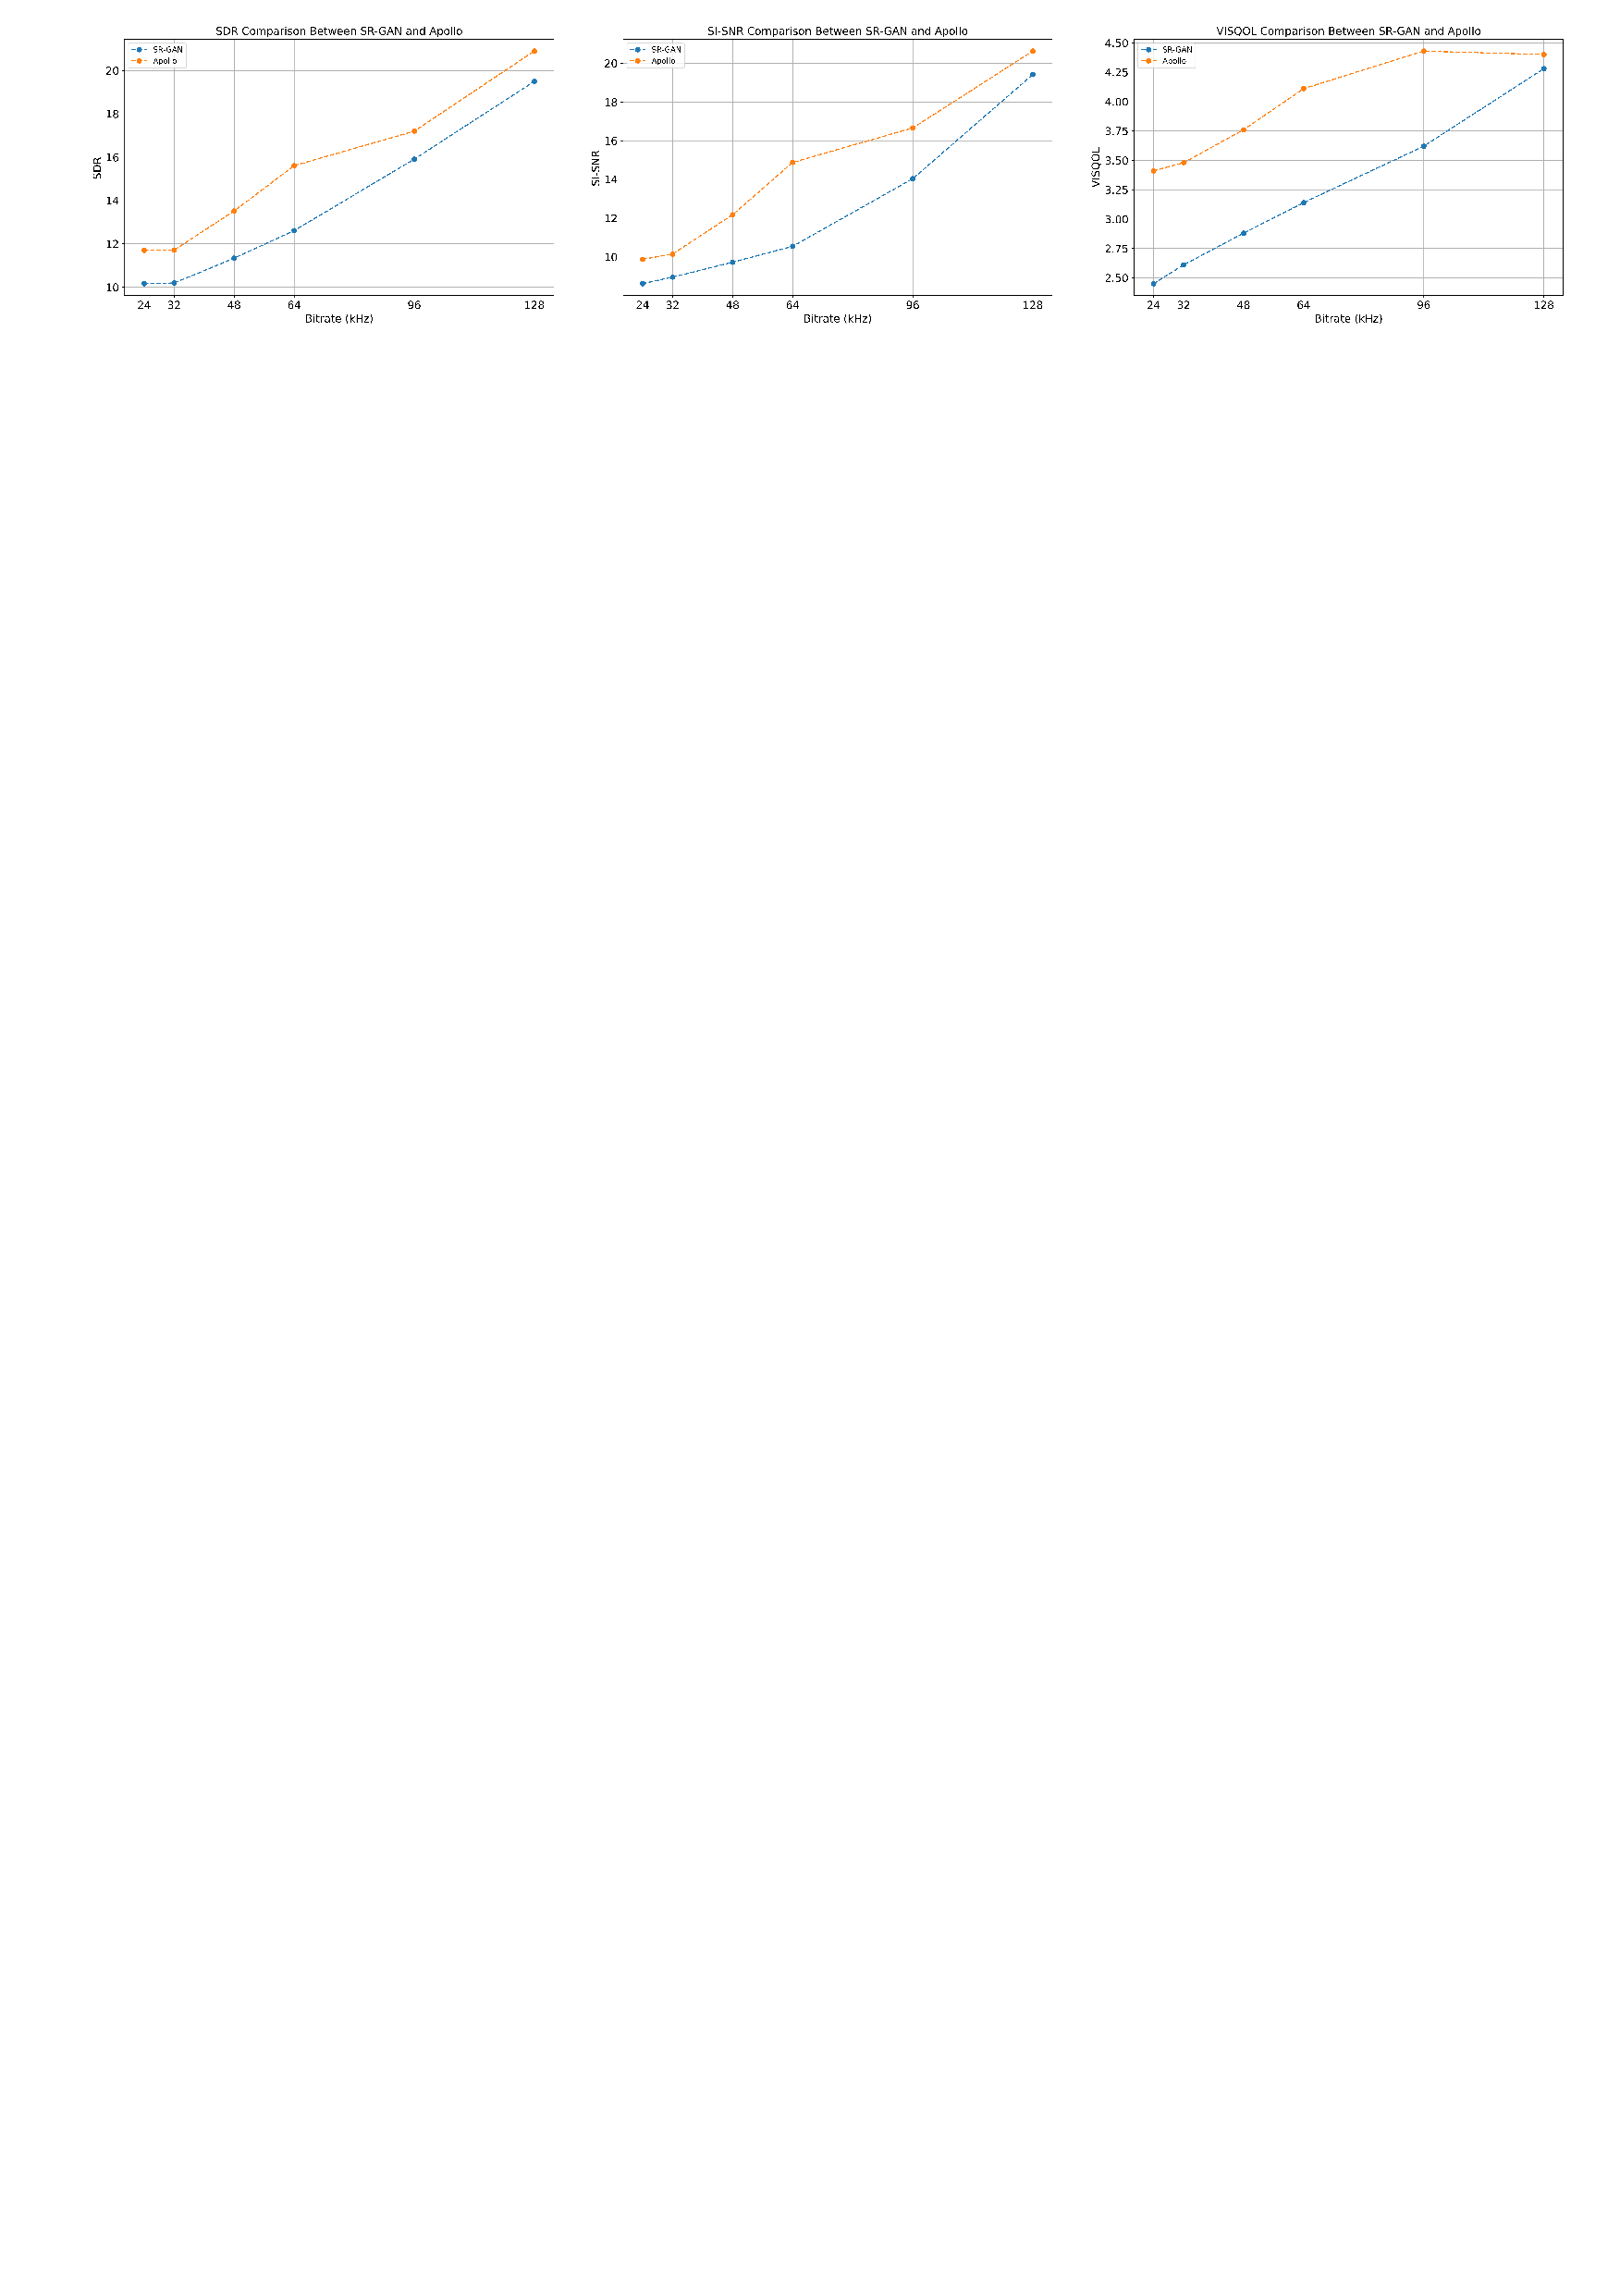
\includegraphics[width=2.0\columnwidth]{Figures/plot.pdf}
	\caption{Apollo and SR-GAN's SDR, SI-SNR and ViSQOL result in comparison at different bitrates.}
	\label{fig:plot}
\end{figure*}

\begin{table*}[]
\footnotesize
\centering
\caption{Different methods' SDR/SI-SNR/VISQOL scores for various types of music, as well as the number of model parameters and GPU inference time. For the GPU inference time test, a music signal with a sampling rate of 44.1 kHz and a length of 1 second was used.}
\begin{tabular}{cccccccc}
\toprule
Model  & Vocal            & Single Stem      & Multi-Stems      & Multi-Stems+Vocal & Overall   & Params (M) & RTF (ms)      \\ \midrule
SR-GAN \cite{lattner2021stochastic} & 10.62/9.19/2.72  & 13.88/12.52/3.28 & 14.92/14.16/3.41 & 16.87/15.54/3.76  & 14.07/12.85/3.29 & 322.53 & \textbf{34.55}\\
Apollo (Ours) & \textbf{13.99/12.58/3.44} & \textbf{16.56/15.99/4.08} & \textbf{17.52/17.15/4.41} & \textbf{18.51/18.26/4.54}  & \textbf{16.64/16.00/4.12} & \textbf{16.54} & 53.23 \\ \bottomrule
\end{tabular}
\label{tab:stems}
\vspace{-10pt}
\end{table*}

\subsection{Training Objection}
The proposed Apollo model is trained using a GAN framework to enhance the quality of audio restoration. Specifically, the discriminator network is inspired by the multi-resolution STFT discriminator, similar to the Gull codec \cite{luo2024gull}. As described in Table \ref{tab:dis}, the discriminator input consists of the spectrogram's real and imaginary parts, which are stacked into a 3D tensor along the channel dimension. To ensure energy invariance in the input, the signal is normalized to have a unit $\ell_2$-norm before being passed into the discriminator. The discriminator is trained using the Least Squares GAN (LSGAN) loss \cite{mao2017least}, defined as:
\begin{equation}
    L_{\text{D}} = \sum_{i=1}^{I}\mathbb{E}_{\mathbf{A} \sim p_{\text{data}}} \left[ (D_i(\mathbf{A}) - 1)^2 \right] + \sum_{i=1}^{I}\mathbb{E}_{\mathbf{Y} \sim p_{\text{G}}} \left[ (D_i(\mathbf{Y}))^2 \right],
\end{equation}
where $\mathbf{A}\in \mathbb{C}^{F\times T}$ denotes the spectrogram of uncompressed audio and $I=5$ denotes the number of discriminator. 

The generator, Apollo, is optimized through a composite loss function, which includes the reconstruction loss, feature matching loss, and the adversarial loss from the discriminator. The \textit{reconstruction loss} $L_{\text{rec}}$ is based on the mean absolute error (MAE) between the magnitude spectrograms of the restored and target audio, evaluated over multiple STFT resolutions:
\begin{equation}
    L_{\text{rec}} =\frac{1}{W} \sum_{w=1}^{W} \frac{\left\| |\text{STFT}_{w}(\mathbf{Y})| - |\text{STFT}_{w}(\mathbf{A})| \right\|_1}{\left\| |\text{STFT}_{w}(\mathbf{T})| \right\|_1 },
\end{equation}
where $\text{STFT}_{w}$ denotes the STFT with window size $w\in [32, 64, 128, 256, 512, 1024, 2048]$. This multi-resolution approach allows the model to capture fine and coarse details, leading to accurate restoration of audio signals across various frequency ranges.

The \textit{feature matching loss} is defined as the layer-wise normalized MAE between the hidden representations of the discriminator for both the reconstructed and target signals. These hidden representations, denoted as $\bar{\mathbf{H}}_{i,j}$ for the reconstructed signal and $\mathbf{H}_{i,j}$ for the target signal, are obtained from the $j$-th layer of the $i$-th discriminator. The feature matching loss is computed as follows:
\begin{equation}
    L_{\text{FM}} = \frac{1}{5} \sum_{i=1}^{5}\left[\frac{1}{6} \sum_{j=1}^{6} \mathbb{E} \left[ \frac{\left| \bar{\mathbf{H}}_{i,j} - \text{sg}[\mathbf{H}_{i,j}] \right|}{\text{mean}\left( \left| \text{sg}[\mathbf{H}_{i,j}] \right| \right)} \right]\right].
\end{equation}

The \textit{reconstruction loss} $L_{\text{rec}}$ is calculated as the multi-resolution frequency MAE over several STFT window sizes, ensuring that both short- and long-term signal characteristics are restored effectively:
\begin{equation}
    L_{\text{rec}} = \frac{1}{W} \sum_{w=1}^{W} \left\| |\text{STFT}_{w}(\mathbf{Y})| - |\text{STFT}_{w}(\mathbf{A})| \right\|_1.
\end{equation}

The overall generator loss combines reconstruction, feature matching, and adversarial losses, expressed as:
\begin{equation}
    L_{\text{G}} = \alpha L_{\text{rec}} + \beta L_{\text{FM}} + \gamma L_{\text{GAN}}
\end{equation}
where $\alpha=1$, $\beta=1$, and $\gamma=1$ are hyperparameters used to balance the contributions of the individual loss components. This comprehensive loss formulation ensures that Apollo reconstructs not only accurate audio signals but also maintains perceptual quality and adversarial robustness by leveraging multi-resolution STFT losses and feature-matching mechanisms.

\section{Experiment configurations}
\label{sec:config}
% Save time on writing our method
\newcommand{\ourmethod}{$\tt{T1}$}

\newcommand{\se}[1]{{\color{magenta} [SE: #1]}}
\newcommand{\fb}[1]{{\color{orange} [FB: #1]}}

\everypar{\looseness=-1}

 \allowdisplaybreaks[4]

\usepackage{tabularx}
\usepackage{fontawesome}

\newcolumntype{\CeX}{>{\centering\let\newline\\\arraybackslash}X}
\newcolumntype{\CeP}{>{\raggedleft\arraybackslash}p}

\newcommand{\TextAndSymbol}[2]{%
  \begin{tabularx}{\textwidth}{X >{\raggedleft}>{\raggedright\arraybackslash}X}%
    #1 & #2
  \end{tabularx}%
}
% \newcommand{\TwoSymbolsAndText}[3]{%
%   \begin{tabularx}{\textwidth}{c\CeX c}%
%     #1 & #2 & #3
%   \end{tabularx}%
% }
% \newcommand{\config}[1]{\TwoSymbolsAndText{\faCogs}{%
%     \textbf{#1}%
%   }{\faCogs}}
\newcommand{\config}[1]{\TextAndSymbol{%
    \textbf{#1}%
  }{\faCogs}}


\usepackage{thmtools} 
\usepackage{thm-restate}

\declaretheorem[name=Theorem,numberwithin=section]{thm}


% Clever references
\usepackage[nameinlink,capitalise]{cleveref}
\crefname{section}{§}{§§}
\Crefname{section}{§}{§§}
\crefname{lemma}{lemma}{lemmas}
\Crefname{lemma}{Lemma}{Lemmas}
\crefname{thm}{theorem}{theorems}
\Crefname{thm}{Theorem}{Theorems}

\title{\textit{Transform Once}\\ Efficient Operator Learning in Frequency Domain}



\section{Results}
\label{sec:result}
\begin{table*}
\small
\centering
\def\arraystretch{1.35}
\begin{tabular}{|l|l|l|l|l|l|}
\hline
      Dimension      & Test & GPT3.5 & GPT4 & Claudev1.3 & Human                         \\ \hline
\multirow{5}{*}{Fluency} & Understandability \& Coherence                                                     &  15.0      & 30.0     &      55.0     &  \textbf{90.0}     \\ \cline{2-6}
 & Narrative Pacing                                                                   &  10.0      &   50.0   &       70.0    &   \textbf{90.0}   \\ \cline{2-6}
 & Scene vs Exposition                                                                &  10.0      &   60.0   &     65.0      &  \textbf{85.0}     \\ \cline{2-6}
 & \begin{tabular}[c]{@{}l@{}}Literary Devices \& Language Proficiency\end{tabular} &   5.0     &   40.0   &     15.0      & \textbf{80.0}      \\ \cline{2-6}
 & Narrative Ending                                                                   & 10.0       & 20.0     &      45.0     &  \textbf{85.0}     \\ \hline\hline
\multirow{3}{*}{Flexibility} & Emotional Flexibility                                                              &   20.0     &  25.0    &    55.0       &  \textbf{90.0}    \\ \cline{2-6}
& Perspective \& Voice Flexibility                                                   &  10.0     &   20.0   &     25.0      &  \textbf{70.0}     \\ \cline{2-6}
& Structural Flexibility                                                             &  15.0      &  30.0    &    35.0       & \textbf{90.0}     \\ \hline\hline
\multirow{3}{*}{Originality} & Originality in Form \& Structure                                                   & 0.0       &   15.0   &     0.0      &  \textbf{60.0}     \\ \cline{2-6}
& Originality in Thought                                                             &   5.0     &   60.0   &     35.0      &  \textbf{90.0}     \\ \cline{2-6}
& Originality in Theme \& Content                                                    &  0.0      &  30.0    &     10.0      &  \textbf{85.0}     \\ \hline\hline
\multirow{3}{*}{Elaboration} &  World Building \& Setting                                                          &   15.0     &   35.0   &    65.0       &  \textbf{90.0}    \\ \cline{2-6}
& Character Development                                                              &   10.0     &  20.0   &  25.0        &  \textbf{75.0}    \\ \cline{2-6}
& Rhetorical Complexity                                                              &    5.0    &  10.0    &    10.0       &  \textbf{90.0}    \\ \hline
\end{tabular}
\vspace{2ex}
\caption{\label{absolutehumaneval}\textbf{Absolute Evaluation}: Average passing rate on individual creativity test obtained from 8 creative writing experts across all stories in our test set authored by GPT3.5,GPT4,Claude and Humans}

\begin{tabular}{|l|l|l|l|l|}
\hline
                                                                               & GPT3.5 & GPT4 & Claudev1.3 & Human \\ \hline
\begin{tabular}[c]{@{}l@{}}Relative Ranking Based on Preference\end{tabular} & 3.45   & 3.0  & 2.35       & 1.2   \\ \hline
\end{tabular}
\vspace{2ex}
\caption{\label{relativehumaneval} \textbf{Relative Evaluation}:Average ranking provided by 8 creative writing experts based on their subjective preference across all stories in our test set authored by GPT3.5,GPT4,Claude and Humans}
\end{table*}

\section{Conclusion}
\label{sec:conclusion}
\section{Conclusion}
\label{sec:conclusion}
This paper introduced \tool, a language to describe distributed machine learning workloads and optimize them across computation and communication boundary. 
We show that \tool{} generated code significantly improves several training and inference times of large language models. 
In the future we plan to automate the optimizations through smart search.

% With ever increasing larger models being trained on massively
% distributed clusters using large datasets, there is a need for
% optimized communication and computation kernels.  Existing techniques
% to improve data-parallel and model-parallel training are limited to a
% particular algorithm, which might not be optimal for different input
% tensor sizes, topology of a distributed system.  In this paper, we
% presented \tool DSL to express programs that contains communication
% and computation and several transformations to optimize these programs
% for wide range of scenarios.  Code generated by \tool performs
% significantly better than hand-optimized state-of-the-arts.


\bibliographystyle{IEEEtran}
\bibliography{refs}

\end{document}
